\chapter{Istzustand}
\label{chapter:Pflichtenheft-Istzustand}

\section{Der Simulator}
\label{section:Pflichtenheft-Istzustand-Simulator}

Vom Auftraggeber ist ein lauffähiger Simulator einer Minimax"=Maschine gegeben. Dieser wird über Textdateien gesteuert, welche die Hardwarekomponenten in einer speziellen Beschreibungssprache definieren. Dazu zählen unter anderem Register, Multiplexer, ALU, CU, Sign, Speicher und Verbindungen. Durch hinzufügen weiterer Steuerungsdateien lässt sich die virtuelle Maschine erweitern.

Der Simulator selbst ist in Java (ab 1.3) realisiert und somit plattformunabhängig. Ein Quellcode liegt nicht vor.

Begleitend ist ein umfangreiches Handbuch in PDF"=Form vorhanden (siehe \cite{minimax-handbuch}), welches alle wichtigen Eigenschaften des Simulators und der Basiskonfiguration erläutert. Weitere Informationen zum Simulator können diesem entnommen werden. Für die Bedienung notwendige Schritte werden später in \autoref{part:Dokumentation} dieser Dokumentation erläutert.

\begin{figure}[htb]
    \centering
    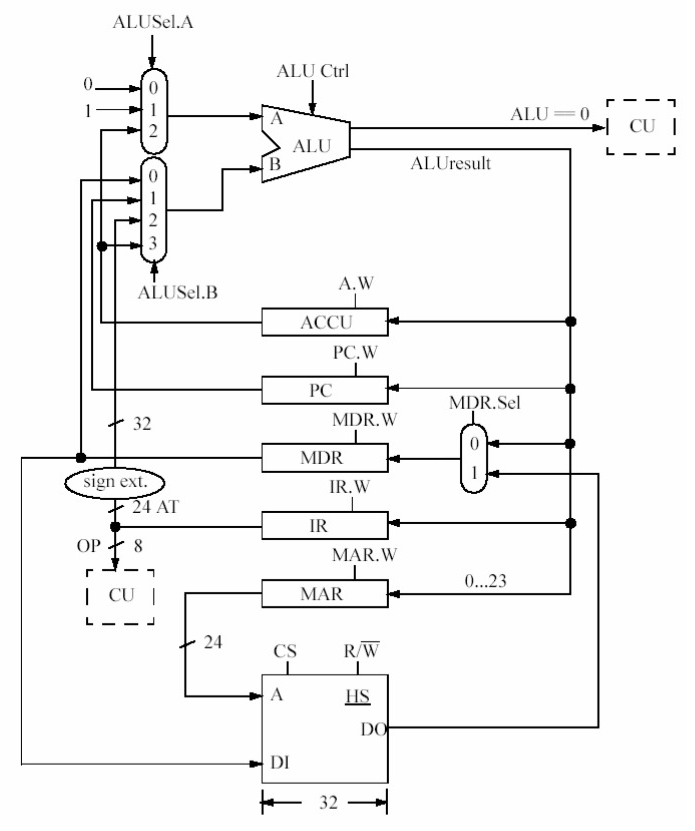
\includegraphics[width=0.7\textwidth]{pflichtenheft/res/minimax.png}
    \caption{Schematische Darstellung der Minimax"=Maschine}
    \label{figure:Pflichtenheft-Istzustand-Simulator-Schema}
\end{figure}

Im Folgenden soll noch die gegebene Basiskonfiguration erläutert werden.

\subsection{Basiskonfiguration}
\label{subsection:Pflichtenheft-Istzustand-Simulator-Basiskonfiguration}

Die Minimax"=Maschine arbeitet vereinfacht ausgedrückt mit einem Datenkreislauf zwischen \emph{Registern} und der \emph{Arithmetic Logic Unit} (ALU), gesteuert durch die \emph{Control Unit} (CU). In der Basiskonfiguration existieren folgende Register (mit ihren jeweilig zugedachten Aufgaben):

\begin{description}
    \item[ACCU] \emph{Accumulator}, Zwischenspeicher
    \item[PC] \emph{Program Counter}, Zähler für Programmablauf
    \item[MDR] \emph{Memory Data Register}, erhält Daten gesteuert durch den Multiplexer \emph{MDR.Sel} (MDR Selector) entweder aus der ALU oder aus dem Hauptspeicher (HS)
    \item[IR] \emph{Instruction Register}, enthält den aktuellen Befehl (8 Bit) mit Adressteil (24 Bit). Der Befehl wird an die CU weitergeleitet. Der Adressteil wird durch die Sign Extension Unit vorzeichenrichtig auf 32 Bit aufgefüllt (\emph{AT}).\todo{verschönern}
    \item[MAR] \emph{Memory Address Register}, enthält die Speicheradresse, aus der Daten vom HS gelesen werden sollen
\end{description}

Jedes Register hat als Eingang mindestens die ALU und besitzt zusätlich einen Steuerungseingang, welcher den Schreibzugriff regelt.

Die ALU wird über den Eingang \emph{ALU.Ctrl} gesteuert und  hat zwei Eingänge, welche mit Multiplexern (gesteuert über \emph{ALUSel.A} und \emph{ALUSel.B}) beschaltet sind. Diese haben folgende Eingänge:

\textbf{A:} 0, 1, ACCU\\
\textbf{B:} MDR, PC, AT, ACCU

In der ALU sind durch die Basiskonfiguration folgende Operationen implementiert, welche durch die oben genannten Multiplexer realisiert sind und über den Eingang ALU.Ctrl gesteuert werden:

\begin{description}
    \item[ADD] $ALUresult \gets A + B$
    \item[SUB.B] $ALUresult \gets -A + B$
    \item[TRANS.A] $ALUresult \gets A$
    \item[TRANS.B] $ALUresult \gets B$
\end{description}

\todo{
\begin{itemize}
    \item Speicherbreite
    \item Speicherzugriff
    \item CU, PC genauer erläutern
\end{itemize}
}


\section{Projektdateien}
\label{section:Pflichtenheft-Istzustand-Projektdateien}

Die Aufgaben und Anforderungen wurden als PDF"=Dokument (siehe \cite{aufgabenblatt}) zur Verfügung gestellt. Einige Punkte daraus werden bei Gelegenheit in diesem Dokument aufgeführt und erläutert. Weitere Informationen zum Projekt befinden sich in einer weiteren PDF (siehe \cite{projektinfo}).

In Bezug auf die Aufgabe sind außerdem Speicherabbilder für einen einheitlichen Benchmark"=Vergleich gegeben. Das Format kann vom Simulator ohne Anpassungen gelesen werden.

